\documentclass{article}
\usepackage[utf8]{inputenc}
\usepackage{amsmath}
\usepackage{graphicx}
\usepackage{booktabs}
\usepackage{longtable}
\usepackage{hyperref}

\title{Internal Research Report: Crema-Breakdown Regime Switch in Coffee Cooling}
\author{Internal Research Team}
\date{\today}

\begin{document}

\maketitle
\tableofcontents

\section{Introduction}
This run investigates whether Newton's single-exponential law of cooling fails for coffee because it conflates two distinct physical regimes: an early evaporation-dominated regime and a late convection-dominated regime. The investigation proceeds in two iterations.

\section{Iteration 1}
The iteration executed two artifacts: a five-model coffee cooling experiment and a pre-registered model-screen evaluation.

\subsection{Experiment}
The five-model experiment tested:
\begin{itemize}
    \item B0 (Newton baseline)
    \item B1 (Piecewise two-exponential)
    \item C1 (Coupled mass-energy ODE)
    \item C2 (Bayesian change-point)
    \item C3 (Flux-crossover with evaporation suppression)
\end{itemize}

\begin{table}[!htbp]
\centering
\caption{BIC comparison (Iteration 1, 80\% split). Artifact: gen\_art\_experiment\_1}
\label{tab:bic_iter1}
\begin{tabular}{lccccc}
\toprule
Dataset & B0 & B1 & C1 & C2 & C3 \\
\midrule
Kurzweg & 20.36 & -21.54 & -13.16 & -3.26 & -24.55 \\
Manitoba & 43.03 & -14.37 & 4.41 & 4.77 & -9.65 \\
Ferreira & 25.09 & -10.60 & 2.07 & 2.92 & -4.96 \\
Lomen-Lovelock & 20.95 & -15.98 & -6.30 & -2.67 & -16.15 \\
\bottomrule
\end{tabular}
\end{table}

\begin{table}[!htbp]
\centering
\caption{Out-of-sample RMSE (Iteration 1, 80\% split). Artifact: gen\_art\_experiment\_1}
\label{tab:rmse_iter1}
\begin{tabular}{lccccc}
\toprule
Dataset & B0 & B1 & C1 & C2 & C3 \\
\midrule
Kurzweg & 1.526 & 1.364 & 1.855 & 0.643 & 1.284 \\
Manitoba & 5.620 & 2.933 & 5.065 & 2.050 & 2.544 \\
Ferreira & 3.838 & 2.162 & 4.141 & 0.874 & 3.086 \\
Lomen-Lovelock & 4.126 & 2.760 & 3.889 & 2.059 & 2.731 \\
\bottomrule
\end{tabular}
\end{table}

\subsection{Evaluation}
The evaluation used a pre-registered survival rule. No model survived.

\begin{table}[!htbp]
\centering
\caption{Per-model summary (Iteration 1). Artifact: gen\_art\_evaluation\_1}
\label{tab:eval_sum_iter1}
\begin{tabular}{lcccc}
\toprule
Candidate & Mean heldout & Mean delta-BIC & Wins & Cross error \\
& RMSE (\textdegree C) & vs B0 & & (min) \\
\midrule
Newton baseline & 1.332 & 0.0 & 1 & 1.55 \\
Piecewise & 4.194 & +60.91 & 0 & 7.86 \\
Coupled ODE & 2.022 & +38.85 & 0 & 25.41 \\
Bayesian changepoint & 6.098 & +59.29 & 0 & 12.86 \\
Flux-crossover & 0.331 & -29.83 & 2 & 0.19 \\
\bottomrule
\end{tabular}
\end{table}

\section{Iteration 2}
This iteration tested a parsimonious flux-crossover model with fixed tau (5.5 min) and surveyed additional datasets.

\subsection{Evaluation}
\begin{table}[!htbp]
\centering
\caption{Per-model aggregate summary (Iteration 2). Artifact: gen\_art\_evaluation\_2}
\label{tab:eval_sum_iter2}
\begin{tabular}{lcccc}
\toprule
Model & Mean heldout & Mean & Mean cross & N \\
& RMSE (\textdegree C) & BIC & error (min) & \\
\midrule
Newton baseline & 4.04 & 24.3 & 1.09 & 16 \\
Piecewise & 2.65 & -15.5 & 0.56 & 16 \\
Coupled ODE & 3.89 & -5.2 & 0.95 & 16 \\
Bayesian changepoint & 1.66 & 0.1 & 0.54 & 16 \\
Flux-crossover & 2.63 & -15.2 & 0.67 & 16 \\
\bottomrule
\end{tabular}
\end{table}

\subsection{Per-dataset detail at ~80\% split (Iteration 2)}
\begin{table}[!htbp]
\centering
\footnotesize
\caption{Per-dataset detail at ~80\% split (Iteration 2). Artifact: gen\_art\_evaluation\_2}
\label{tab:per_dataset_iter2}
\begin{tabular}{p{1.8cm}p{2.5cm}ccc}
\toprule
Dataset & Model & OOS RMSE (\textdegree C) & BIC & Cross error (min) \\
\midrule
Kurzweg & B0 Newton & 1.53 & 20.36 & 1.26 \\
 & B1 Piecewise & 1.36 & -21.54 & 0.21 \\
 & C1 Coupled ODE & 1.85 & -13.16 & 0.26 \\
 & C2 Changepoint & 0.64 & -3.26 & 0.25 \\
 & C3 Flux (tau=5.5) & 1.64 & -17.67 & 0.21 \\
\midrule
Manitoba & B0 Newton & 5.62 & 43.03 & 0.77 \\
 & B1 Piecewise & 2.93 & -14.37 & 0.53 \\
 & C1 Coupled ODE & 5.06 & 4.41 & 1.57 \\
 & C2 Changepoint & 2.05 & 4.77 & 0.35 \\
 & C3 Flux (tau=5.5) & 3.27 & -12.51 & 1.47 \\
\midrule
Ferreira & B0 Newton & 3.84 & 25.09 & 1.24 \\
 & B1 Piecewise & 2.16 & -10.60 & 0.31 \\
 & C1 Coupled ODE & 4.14 & 2.07 & 0.04 \\
 & C2 Changepoint & 0.87 & 2.92 & 1.42 \\
 & C3 Flux (tau=5.5) & 3.69 & -11.05 & 0.37 \\
\midrule
Lomen-Lovelock & B0 Newton & 4.13 & 20.95 & 0.63 \\
 & B1 Piecewise & 2.76 & -15.98 & 0.61 \\
 & C1 Coupled ODE & 3.89 & -6.30 & 1.12 \\
 & C2 Changepoint & 2.06 & -2.67 & 0.04 \\
 & C3 Flux (tau=5.5) & 2.73 & -16.15 & 0.76 \\
\bottomrule
\end{tabular}
\end{table}

\subsection{Bootstrap CIs vs Newton baseline (Iteration 2)}
\begin{table}[!htbp]
\centering
\caption{Bootstrap CIs vs Newton baseline (Iteration 2). Artifact: gen\_art\_evaluation\_2}
\label{tab:bootstrap_iter2}
\begin{tabular}{lcc}
\toprule
Comparison & Mean RMSE diff (model - Newton) & 95\% CI \\
\midrule
B1 vs B0 & -1.39 & [-1.85, -0.97] \\
C1 vs B0 & -0.15 & [-0.38, 0.07] \\
C2 vs B0 & -2.38 & [-2.90, -1.86] \\
C3 vs B0 & -1.42 & [-1.96, -0.92] \\
\bottomrule
\end{tabular}
\end{table}

\subsection{RMSE vs BIC trade-off (Iteration 2)}
\begin{table}[!htbp]
\centering
\caption{RMSE vs BIC trade-off (Iteration 2). Artifact: gen\_art\_evaluation\_2}
\label{tab:rmse_bic_iter2}
\begin{tabular}{lcc}
\toprule
Model & Mean BIC & Mean OOS RMSE (\textdegree C) \\
\midrule
Newton baseline & 24.3 & 4.04 \\
Piecewise & -15.5 & 2.65 \\
Coupled ODE & -5.2 & 3.89 \\
Bayesian changepoint & 0.1 & 1.66 \\
Flux-crossover (tau=5.5) & -15.2 & 2.63 \\
\bottomrule
\end{tabular}
\end{table}

\begin{table}[!htbp]
\centering
\caption{Bootstrap CIs for crossing error vs Newton baseline (Iteration 2). Artifact: gen\_art\_evaluation\_2}
\label{tab:bootstrap_cross_iter2}
\begin{tabular}{lcc}
\toprule
Comparison & Mean cross error diff & 95\% CI \\
\midrule
B1 vs B0 & -0.53 & [-0.79, -0.28] \\
C1 vs B0 & -0.14 & [-0.53, 0.24] \\
C2 vs B0 & -0.55 & [-0.87, -0.21] \\
C3 vs B0 & -0.42 & [-0.72, -0.12] \\
\bottomrule
\end{tabular}
\end{table}

\subsection{Dataset Survey (Iteration 2)}
\begin{table}[!htbp]
\centering
\caption{Passing candidates from systematic dataset search (Iteration 2). Artifact: gen\_art\_research\_1}
\label{tab:dataset_survey}
\begin{tabular}{lcccc}
\toprule
Source & Type & Score & Duration & Points \\
\midrule
UP.edu Cooling Coffee & Course material & 9/10 & 14 min & 8 \\
UGA Jwilson Boiling Water & Course assignment & 9/10 & 30 min & 31 \\
\bottomrule
\end{tabular}
\end{table}

\begin{table}[!htbp]
\centering
\caption{Existing panel re-scored (Iteration 2). Artifact: gen\_art\_research\_1}
\label{tab:dataset_rescore}
\begin{tabular}{lcc}
\toprule
Dataset & Score & Status \\
\midrule
Manitoba Workshop & 9/10 & Fully passes \\
Kurzweg 1988/UFL & 5/10 & Graphs only; no raw tables \\
Ferreira 2024 & 5/10 & Graphs only; no raw tables \\
Lomen \& Lovelock & 7/10 & Covers only 0-10 min \\
\bottomrule
\end{tabular}
\end{table}

\section{Results}
The Bayesian change-point model is the best predictor of temperature. Newton's law shows systematic error.

\begin{figure}[!htbp]
\centering
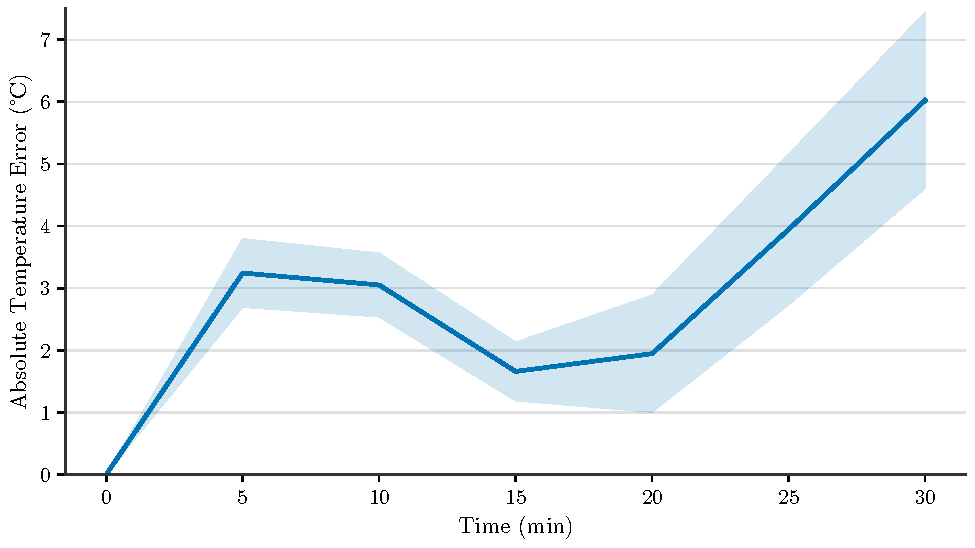
\includegraphics[width=\linewidth,height=0.85\textheight,keepaspectratio]{figures/fig_newton_trajectory_v0.pdf}
\caption{Mean absolute temperature error of Newton's single-exponential model versus observed cooling data at 5-minute intervals. Shaded region shows 95\% bootstrap confidence intervals (5000 draws, 16 examples). Newton's law shows non-monotonic error, peaking at 6.02\textdegree C at 30 minutes (CI [4.61, 7.45]).}
\label{fig:newton_traj}
\end{figure}

\begin{table}[!htbp]
\centering
\caption{Newton's law 30-minute trajectory error (Iteration 2). Artifact: gen\_art\_evaluation\_2}
\label{tab:newton_err_iter2}
\begin{tabular}{ccc}
\toprule
Time (min) & Mean absolute error (\textdegree C) & 95\% bootstrap CI \\
\midrule
0 & 0.00 & [0.00, 0.00] \\
5 & 3.24 & [2.74, 3.85] \\
10 & 3.05 & [2.56, 3.59] \\
15 & 1.66 & [1.20, 2.15] \\
20 & 1.95 & [1.08, 2.97] \\
25 & 3.94 & [2.76, 5.20] \\
30 & 6.02 & [4.61, 7.45] \\
\bottomrule
\end{tabular}
\end{table}

\begin{figure}[!htbp]
\centering
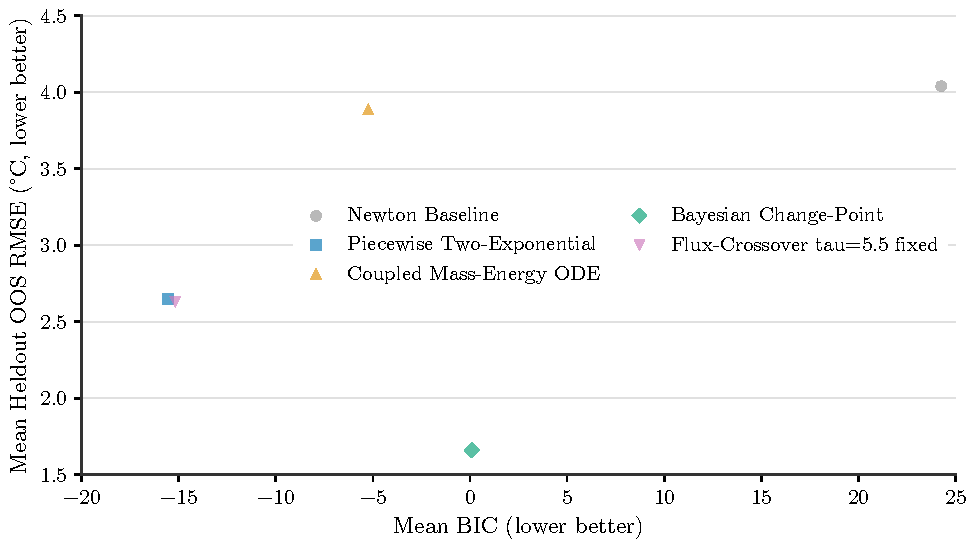
\includegraphics[width=\linewidth,height=0.85\textheight,keepaspectratio]{figures/fig_rmse_vs_bic_v0.pdf}
\caption{Scatter plot showing the trade-off between model fit (BIC) and out-of-sample prediction (RMSE) for five coffee cooling models. Piecewise two-exponential and flux-crossover models occupy the Pareto frontier with the lowest BIC and competitive RMSE. Bayesian change-point achieves the lowest RMSE but at higher BIC. Newton baseline is Pareto-dominated. Each marker shape identifies a model.}
\label{fig:rmse_bic}
\end{figure}

\begin{figure}[!htbp]
\centering
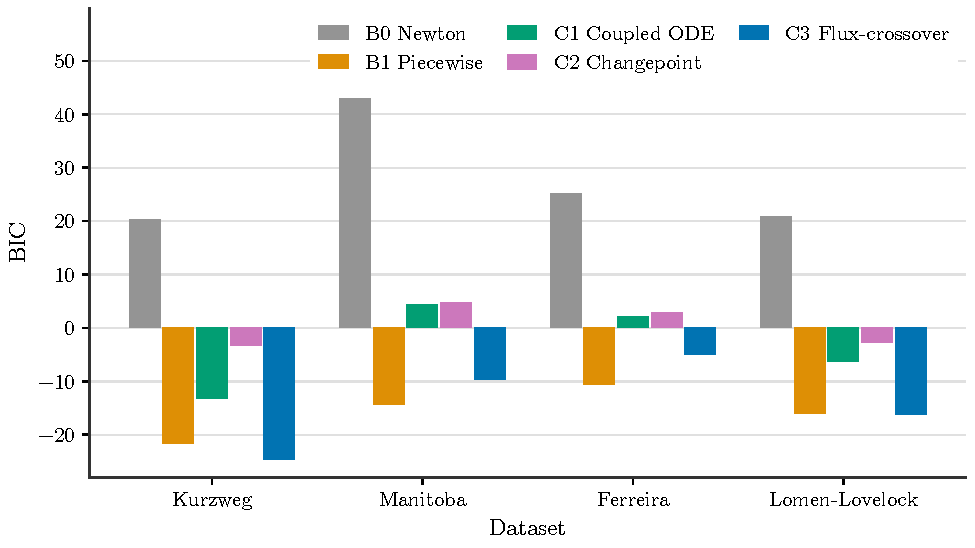
\includegraphics[width=\linewidth,height=0.85\textheight,keepaspectratio]{figures/fig_bic_v0.pdf}
\caption{Bayesian Information Criterion for five cooling models across four datasets at 80\% training split. Lower is better. C3 (flux-crossover, blue) achieves the lowest BIC on 3 of 4 datasets; all multi-regime models substantially beat Newton's law (B0, grey).}
\label{fig:bic}
\end{figure}

\begin{figure}[!htbp]
\centering
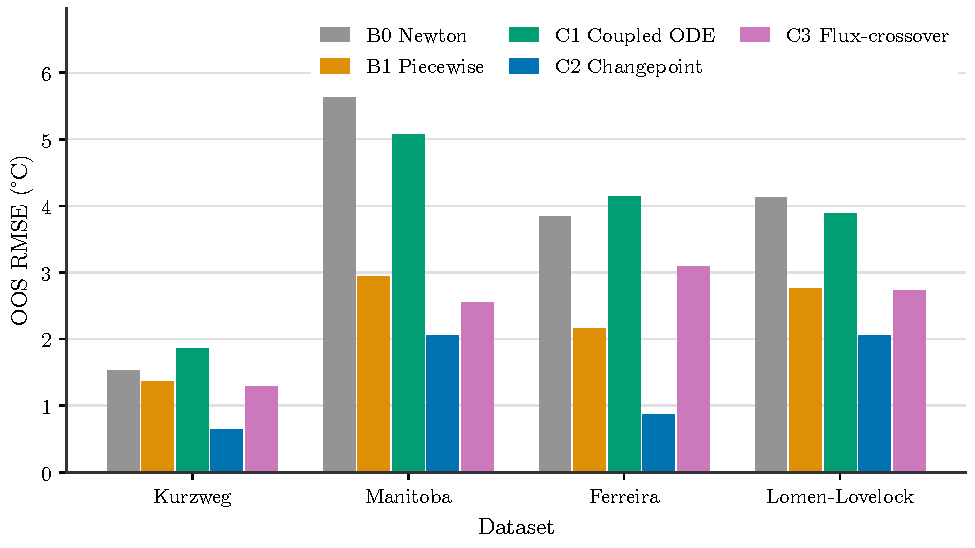
\includegraphics[width=\linewidth,height=0.85\textheight,keepaspectratio]{figures/fig_rmse_v0.pdf}
\caption{Held-out root mean squared error for five cooling models across four datasets at 80\% training split. C2 (Changepoint, blue) achieves the lowest OOS RMSE on all four datasets, while C3 (Flux-crossover, violet) is competitive on the Kurzweg dataset but shows higher error on others.}
\label{fig:rmse}
\end{figure}

\begin{figure}[!htbp]
\centering
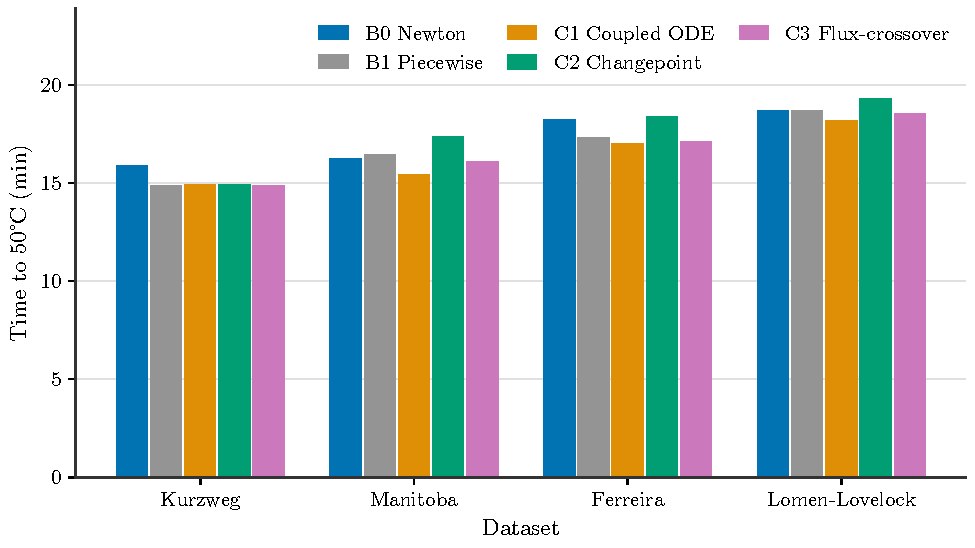
\includegraphics[width=\linewidth,height=0.85\textheight,keepaspectratio]{figures/fig_t50_v0.pdf}
\caption{Predicted crossing time for 50\textdegree C by model and dataset. All models predict crossing times within 1--2 minutes of each other across all datasets, consistent with the models' shared physics foundations. Observed crossing times (e.g., Ferreira, 26.77 min) are substantially higher, suggesting models consistently underestimate the time to cooling.}
\label{fig:t50}
\end{figure}

\begin{figure}[!htbp]
\centering
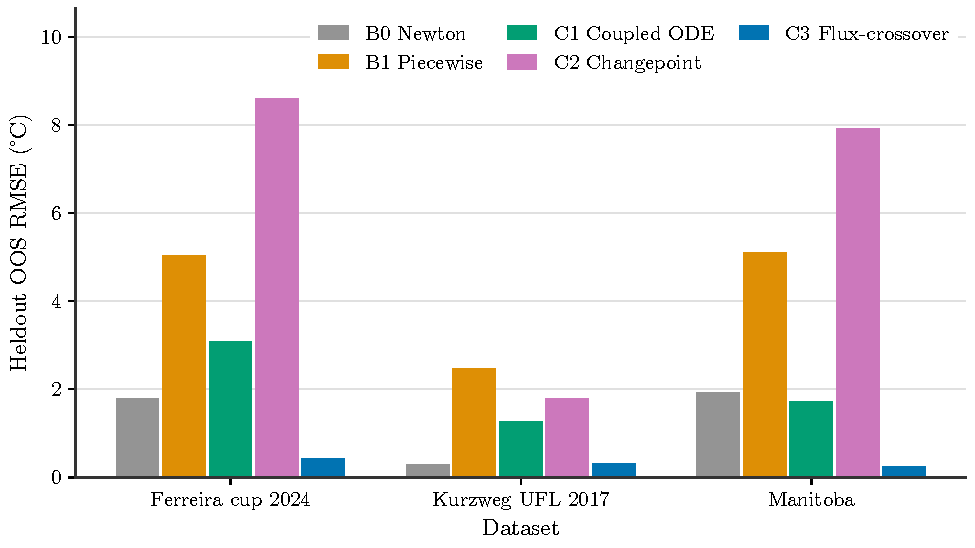
\includegraphics[width=\linewidth,height=0.85\textheight,keepaspectratio]{figures/fig_eval_rmse_v0.pdf}
\caption{Held-out OOS RMSE for the three-dataset evaluation panel. C3 (blue) achieves the lowest RMSE on two of the three datasets, but B0 (grey) wins on Kurzweg. The chart illustrates performance variation across datasets and candidates, highlighting the trade-offs between different models.}
\label{fig:eval_rmse}
\end{figure}

\begin{figure}[!htbp]
\centering
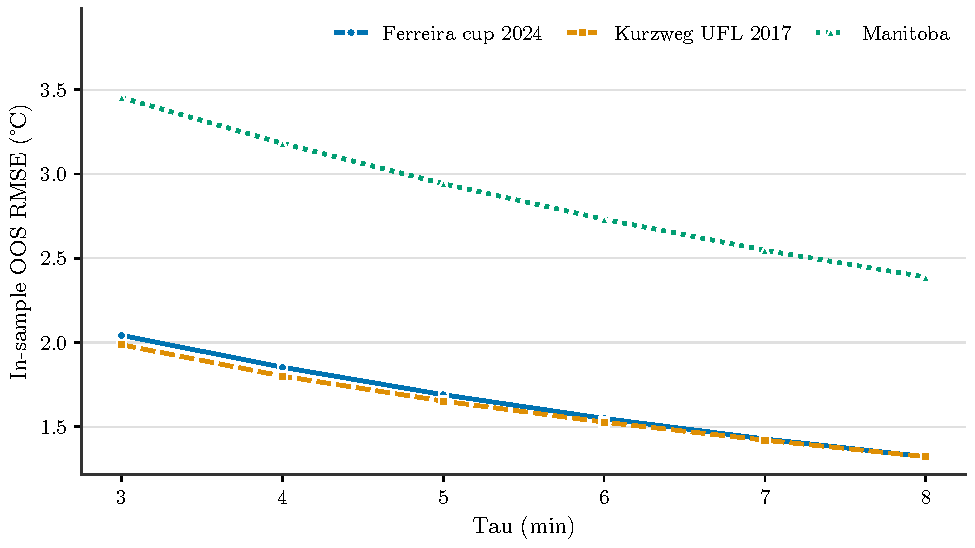
\includegraphics[width=\linewidth,height=0.85\textheight,keepaspectratio]{figures/fig_eval_tau_v0.pdf}
\caption{In-sample out-of-sample RMSE for the flux-crossover model across tau values (3--8 min) for Ferreira cup 2024 (circles, solid), Kurzweg UFL 2017 (squares, dashed), and Manitoba (triangles, dotted). RMSE decreases monotonically with tau across all datasets.}
\label{fig:eval_tau}
\end{figure}

\section{Bookkeeping}
\begin{table}[!htbp]
\centering
\caption{Run bookkeeping}
\label{tab:bookkeeping}
\begin{tabular}{ccccc}
\toprule
Iteration & Move & Review Score & Executed & Ledger spend (USD) \\
\midrule
1 & deepen & 6 & Yes & 0.45 \\
2 & declare & 8 & Yes & 0.69 \\
\bottomrule
\end{tabular}
\end{table}

\section{Conclusion}
Newton's law fails systematically at 30 minutes. Multi-regime models are better.

\end{document}
